\chapter{Results}
This section discusses measurement accuracy and the speed of the code.

\section{Measurement accuracy}
Both the length ($L$) and the diameter ($D$) of a the steel spring, which is the object to be measured in the industry, have been measured.

300 measurements were taken with no movement, or respectively static and again 300 measurements with a moving object.
For these dynamic measurements, the demonstrator has to be tilted until the angle between the glass plate and the horizontal is 15 degrees.
The object velocity in the horizontal direction, used for the rolling shutter correction, is estimated as 2\,m/s.
Unfortunately, the implemented trigger has it's given limitations and does not work with higher velocities.

The histograms are shown in Figure \ref{development:hist}.
The static measurements are plotted in orange and the dynamic in blue.
The label displays each mean ($\mu$) and standard deviation ($\sigma$).
\begin{figure}[ht]
	\centering
	\subfigure[\label{development:hist1}]{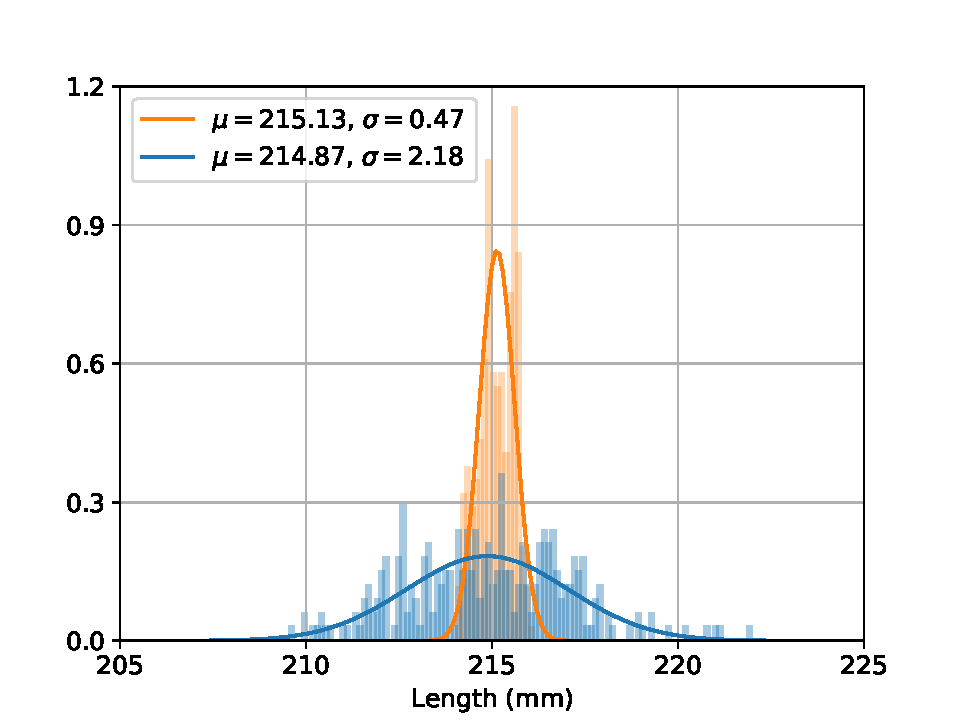
\includegraphics[width=0.45\linewidth]{4-results/images/hist_length.pdf}}
	\subfigure[\label{development:hist2}]{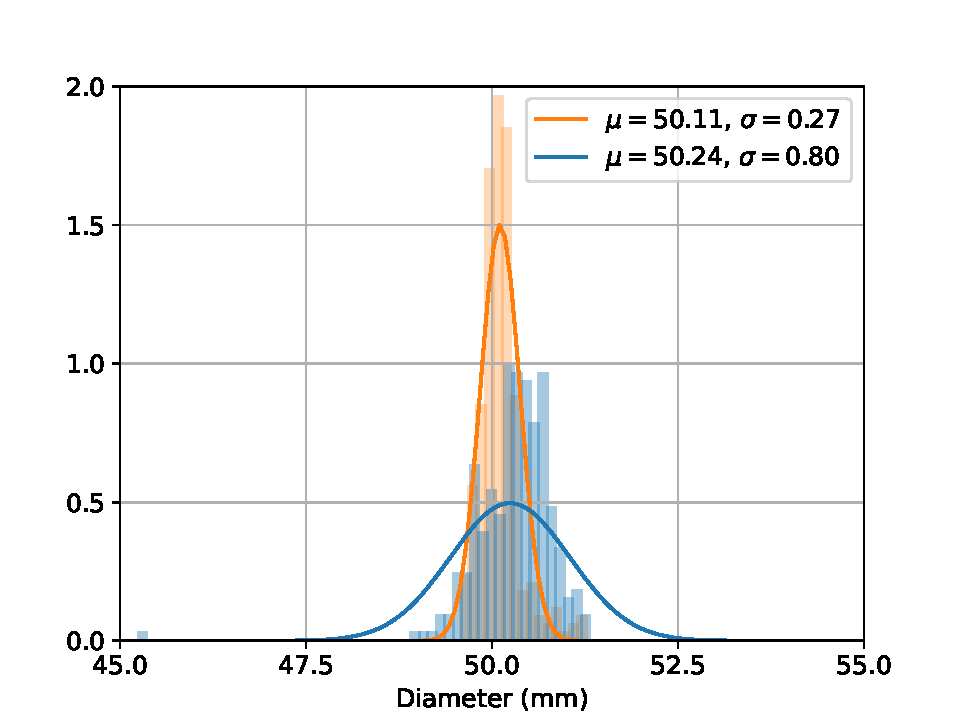
\includegraphics[width=0.45\linewidth]{4-results/images/hist_diameter.pdf}}
	\caption{Histograms of both the dynamic and static measurements\label{development:hist}}		
\end{figure}
The static and dynamic mean of the length is very similar, which indicates that the assumption that the spring moves at a speed of 2\,m/s is valid.

The relative errors are computed like
\begin{align*}
	e_{L}^{\text{static}}&=\frac{0.47}{215.13}=0.22\%&e_D^{\text{static}}&=\frac{0.27}{50.11}=0.54\%\\
	e_{L}^{\text{dynamic}}&=\frac{2.18}{214.87}=1.01\%&e_D^{\text{dynamic}}&=\frac{0.8}{50.24}=1.60\%.
\end{align*}


\section{Speed}